% A short introduction on Make.

\documentclass[12pt, letterpaper]{article}

\usepackage{graphicx}
\usepackage{anysize}
\marginsize{.5in}{.5in}{.5in}{.5in}

\begin{document}
%%%%%%%%%%%%%%%%%%%%%%%%%%%%%%%%%%%%%%%%%%%%%%%%%%%%%%%%%%%%%%%%%%%%%%%%%%%%%%
\begin{center}
  {\LARGE \textbf{GNU Make: A Crash Course}}\\
  D. T. Welling (dwelling@umich.edu)
\end{center}

GNU Make is a utility to \emph{build} complicated things, like programs or
\LaTeX documents.  It is designed to handle goals that have a clear
hierarchy of tasks, i.e. each step has \emph{prerequisites} that must be
completed before advancing.  Make is especially useful when developing code
because at each step, it determines if all prerequisites need to be re-built
or if some are \emph{up-to-date}.  To use make, a user must first write a
\emph{Makefile}, which must be called {\tt Makefile}.  
Then, the user simply invokes Make by typing {\tt make} at the command prompt.

\begin{center}
  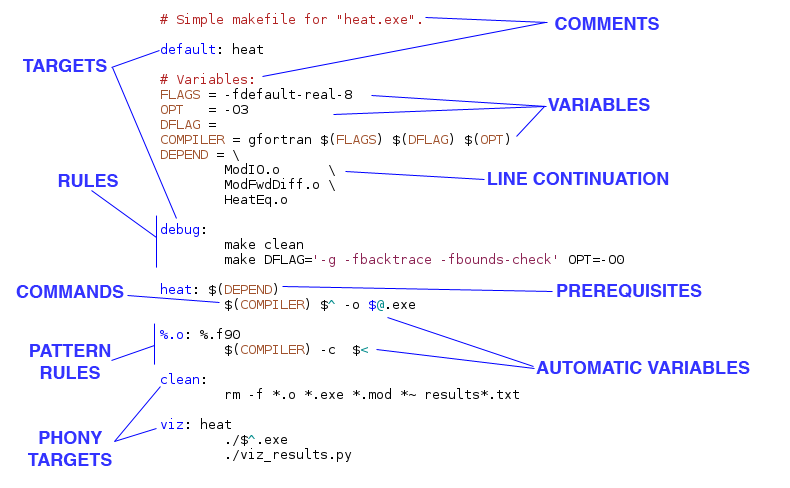
\includegraphics[width=6.5in]{make_diagram.png}
\end{center}

\noindent \textbf{Rules:} The most basic part of a Makefile is a \emph{rule}.
This is a block of text that specifies a goal, or \emph{target}, any 
\emph{prerequisites} required to build the target, and what 
\emph{commands} must be executed to create the target.  The first
target in the file becomes the \emph{default} and is the one that is made
by typing {\tt make} with no arguments.  Other targets can be selected by
using arguments.  For example, typing {\tt make clean} will build the 
target ``clean'' instead of ``default'' in the above example.

\vspace{0.5cm}

\noindent \textbf{Targets:} \emph{Targets} are the end goal of each
individual rule.  Typically, a target is the name of a file that will be 
created once the rule's commands are executed, but \emph{phony targets}, 
targets that do not refer to explicit files, are also acceptable.  When
a rule is executed, Make investigates to see if the target is \emph{up-to-date}.
This is true if the file the target refers to exists, is more recent than
any prerequisites that are files, and all of the prerequisites that are also
targets are up-to-date.  This checking system is how Make minimizes the 
work performed when building targets.  Note that phony targets are
always considered out-of-date.

There are many ``standard'' phony targets, i.e. targets that users of
your Makefile will expect to exist.  The most important of these is {\tt clean}.
It is standard that {\tt make clean} will remove all intermediate files and
return the status of the build to its original state.  You should always
include {\tt clean} in your file and give it meaningful clean-up tasks to
perform.

\vspace{0.5cm}

\noindent \textbf{Prerequisites:} \emph{Prerequisites} (alternatively, 
\emph{dependencies}) can be explicitly listed files or other targets.  If it
is a file that does not exist, Make will search for a target that has the
same file name or matches a \emph{pattern rule} and execute that rule.  All
prereqs of a target must be up-to-date before the target can be built.

\vspace{0.5cm}

\noindent \textbf{Commands:} \emph{Commands} follow the {\tt target:prereq}
syntax in a Makefile.  They must be tabbed to the right of the target
declaration.  Commands are just that: any command that you would
explicitly type at your terminal's prompt.  Be sure to use 
\emph{line continuation characters} if a single command wraps over more than
one line.  Make commands are most powerful when combined with regular and
automatic \emph{variables}.

\vspace{0.5cm}

\noindent \textbf{Variables:} \emph{Variables} are key to Make's flexibility.
They are declared very simply: {\tt VAR = value}; it is standard to 
capitalize variable names.  Their values can be any string of characters, there
are very few limits.  To use the value of a variable (known as 
\emph{dereferencing} a variable), the syntax {\tt \verb|$|(VAR)} is used.  
It is possible to use curly braces instead of parentheses based on preference.
When a variable is dereferenced, the value of variable takes the place of the
dereferencing syntax.  In our example, the value of {\tt DEPEND} is
a list of object files ({\tt *.o}-files), split over several lines using the
\emph{line continuation character} for clarity.  This variable is used
later, as a prerequisite to the {\tt heat} target.  Because it is dereferenced
there, the list of files is placed in its stead and each of those files is
understood by Make to be a prerequisite to that target.  It is proper to
use variables to organize your makefile!
Variables can be set at the command line as follows: 
{\tt make DEPEND=otherfile.o}.  This would override the value of {\tt DEPEND}
for the current execution of Make.  Many Makefiles will require you to set
variables at the command line to customize the build.  Always read and include
documentation!

\vspace{0.5cm}

\noindent \textbf{Automatic Variables}: Make has a set of special variables
called \emph{automatic variables}.  Here are the most important ones:
\begin{center}
  \begin{tabular}{|c|l|}
    \hline
    Variable & Meaning \\
    \hline
    \verb|$@| & The filename representing the target.\\ 
    \verb|$<| & The filename of the first prerequisite.\\
    \verb|$?| & A space separated list of all prerequisites 
    newer than the target.\\
    \verb|$^| & A space separated list of all prerequisites, no duplicates.\\
    \verb|$*| & The target filename without its suffix (the stem).
    \emph{Only use inside of pattern rules!}\\
    \hline
  \end{tabular}
\end{center}

\vspace{0.5cm}

\noindent \textbf{Pattern Rules}: It quickly becomes apparent that many 
different prerequisites will have nearly identical
rules.  \emph{Pattern rules} (also known as \emph{implicit rules})
 allow users to combine multiple rules together.
In the example, the rule \verb|%.o| applies to any file that ends in {\tt .o}
that does not have its own \emph{explicit rule}.  
The {\tt\%} symbol acts like a Linux wildcard (*).  The dependency for
this rule is \verb|%.f90|, which means the same file name as the target, but
{\tt .f90} instead of {\tt .o}.  Pattern rules make large builds with
thousands of source files completely feasible with Make.  Note that there
are some built-in pattern rules, most notably \verb|%.o: %.c|.

\vspace{0.5cm}

\noindent \textbf{What does \emph{this} Makefile do?}  The Makefile diagrammed
above
is designed to compile the source file {\tt HeatEq.f90}, which depends on 
{\tt ModFwdDiff.f90} and {\tt ModIO.f90}.  This code models the heat
equation and prints output to an ASCII file.  The output can be visualized
with a Python script, {\tt viz\_results.py}.  All files are assumed to
be in the same directory as the Makefile.

 When called for the first time with no
targets and no variables (i.e., simply ``{\tt make}''), Make looks for the
first target, which is {\tt default}.  It is a \emph{phony target} with
the \emph{prerequisite} {\tt heat}.  There is no file called {\tt heat}, so Make
looks for a rule for this prereq and finds the target with the same name.
The prereqs for target {\tt heat} are given by the \emph{dereferenced variable}
{\tt DEPEND}, which is a list of object files (files ending in {\tt .o}).
Make looks for these files in order, and, of course, will not find them.  It
also finds no \emph{explicit rules} for any of the files.  However, there is
an \emph{implicit pattern rule} for files that end in \verb|.o| whose prereq
is the same file that ends in \verb|.f90|.  This rule's commands are now
executed once for each \verb|*.o| file required by target {\tt heat} in the
order they are listed.
 The \emph{variable} \verb|$(COMPILER)| \emph{dereferences} into 
\verb|gfortran $(FLAGS) $(DFLAG) $(OPT)| which further dereferences into
\verb|gfortran -fdefault-real-8   -O3|.  The \emph{automatic variable}
\verb|$<| dereferences into the FORTRAN filename corresponding to the current
target.  By dereferencing all variables, it becomes clear that this rule is 
compiling each FORTRAN source file into individual object files.

Once all of the {\tt heat} target's prereqs are ready, the {\tt heat} rule's
single command will be executed.  \verb|$(COMPILER)| dereferences the same
as above, \verb|$^| dereferences into a list of prerequisites as set by the
variable {\tt DEPEND}, and \verb|$@.exe| becomes the name of our final
executable, {\tt heat.exe}.  With the final program compiled and linked to
its dependencies, Make is finished.  Here are the
 set of commands explicitly executed:
\begin{verbatim}
gfortran -fdefault-real-8  -O3 -c  ModIO.f90
gfortran -fdefault-real-8  -O3 -c  ModFwdDiff.f90
gfortran -fdefault-real-8  -O3 -c  HeatEq.f90
gfortran -fdefault-real-8  -O3 ModIO.o ModFwdDiff.o HeatEq.o -o heat.exe
\end{verbatim}

There are additional targets that add more functionality.  If the user
calls {\tt make debug}, the phony target {\tt debug} is called instead of
the default.  This target has no prereqs, so the commands are executed without
detour.  First, make calls itself (yes, you can do this!) with the phony
target {\tt clean}.  This phony target merely removes all intermediate files
produced by a single call to Make.  Then, Make calls itself again, but this time
two variables are set to non-default values.  {\tt DFLAG} is set from nothing
to a list of compiler debug flags, and {\tt OPT} is set to the no-optimization
flag.  The target {\tt heat} is then remade using the new variable values.  
The commands executed are as follows:

\begin{verbatim}
rm -f *.o *.exe *.mod *~ results*.txt
make DFLAG='-g -fbacktrace -fbounds-check' OPT=-O0
gfortran -fdefault-real-8 -g -fbacktrace -fbounds-check -O0 -c  ModIO.f90
gfortran -fdefault-real-8 -g -fbacktrace -fbounds-check -O0 -c  ModFwdDiff.f90
gfortran -fdefault-real-8 -g -fbacktrace -fbounds-check -O0 -c  HeatEq.f90
gfortran -fdefault-real-8 -g -fbacktrace -fbounds-check -O0 \
    ModIO.o ModFwdDiff.o HeatEq.o -o heat.exe 
\end{verbatim}

Finally, there is the target {\tt viz}.  This target has {\tt heat} as a 
prereq, so the code is compiled with default variable settings first.  Then,
\verb|./$^.exe| dereferences to {\tt heat.exe}, so the first command for
rule {\tt viz} is to
execute the code that was just compiled.  The next line executes the Python
script, visualizing the results from the simulation.  Within
a single Makefile, a lot of functionality can be stored.

This guide is a very simple introduction.  The material was taken from 
\emph{Managing Projects from GNU Make, 3rd Ed.} by Robert Mecklenburg.  There
is much more to Make; users are encouraged to continue to explore this 
powerful utility.
%%%%%%%%%%%%%%%%%%%%%%%%%%%%%%%%%%%%%%%%%%%%%%%%%%%%%%%%%%%%%%%%%%%%%%%%%%%%%%
\end{document}
